\section{Aplikace první a druhé derivace}

\subsection{Lineární a kvadratická aproximace}

Hlavní význam derivací spočívá v tom, že pokud pro dané funkce existují (o takových funkcích říkáme, že jsou \uv{dostatečně hladké}), můžeme pomocí nich funkce lokálně aproximovat.
Představme si funkci $f(x)$, která má první i druhou derivaci. Uvažujme nějaký \textbf{pevný bod $x_0$}. Na jeho \textbf{malém okolí} můžeme funkci aproximovat přímkou
\begin{align}
    \boxed{ T_1(x) = f(x_0) + f'(x_0) \cdot (x-x_0) }
\end{align}
anebo parabolou
\begin{align}
    \boxed{ T_2(x) = f(x_0) + f'(x_0) \cdot (x-x_0) +\frac{f''(x_0)}{2}  \cdot (x-x_0)^2 }\:.
\end{align}

\begin{example}
    Aproximujme funkci $f(x) = \sin(x)$ okolo bodu $x_0 = \pi/4$. Platí $f'(x) = \cos (x)$ a $f''(x) = - \sin (x)$, takže $f(\pi/4) = \sin (\pi/4) = \sqrt{2}/2$, $f'(\pi/4) = \cos (\pi/4) = \sqrt{2}/2$ a $f''(\pi/4) = - \sin (\pi/4) = -\sqrt{2}/2$.
    Na nějakém malém okolí tedy můžeme aproximovat přímkou \begin{align}
        T_1(x) = \frac{\sqrt{2}}{2} + \frac{\sqrt{2}}{2} \left(x - \frac{\pi}{4} \right)
    \end{align} 
    a také parabolou
    \begin{align}
        T_2(x) = \frac{\sqrt{2}}{2} + \frac{\sqrt{2}}{2} \left( x - \frac{\pi}{4} \right) 
        - \frac{\sqrt{2}}{4} \left( x - \frac{\pi}{4} \right)^2  \:.
    \end{align}
    Jak je aproximace přesná, ukazuje obrázek \ref{fig:aproximace}.
    \begin{figure}[H]
        \centering

        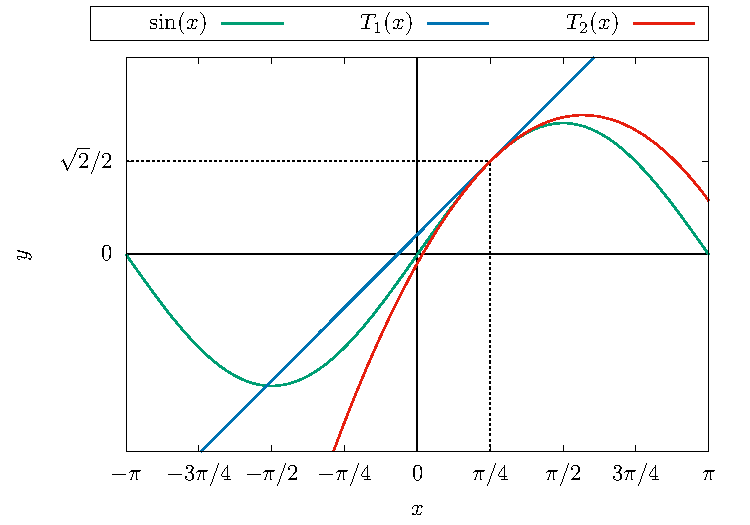
\includegraphics[scale = 0.7]{Gnuplot/Figures/aproximace-sinus.pdf}
        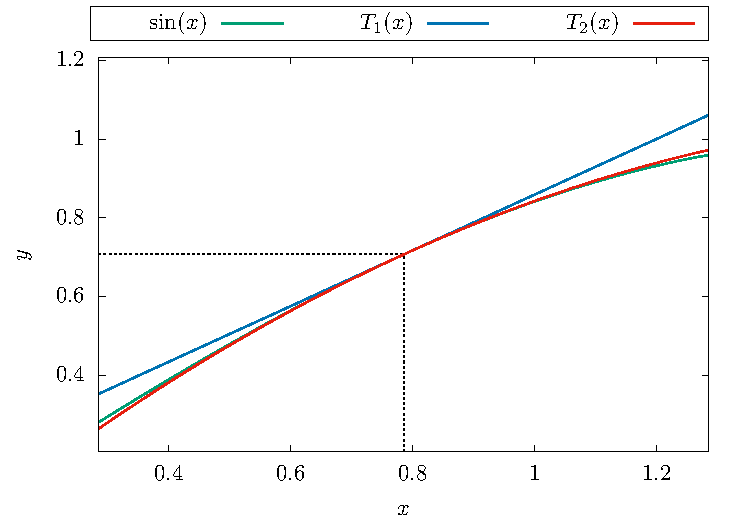
\includegraphics[scale = 0.7]{Gnuplot/Figures/aproximace-sinus2.pdf}
        
        \caption{Aproximace funkce $\sin x$ přímkou $T_1(x)$ a parabolou $T_2(x)$ kolem bodu $\frac{\pi}{4}$.}
        \label{fig:aproximace}
    \end{figure}

\end{example}

\begin{example}
    Pomocí aproximace spočítejme $\sqrt{14}$. Víme, že $\sqrt{16} = 4$. Zkusme proto odmocninu aproximovat kolem bodu $4$. Platí \begin{align}
        (\sqrt{x})' = \frac{1}{2 \sqrt{x}} \:, \quad (\sqrt{x} )'' = -\frac{3}{2 \sqrt{x^3}} \:.
    \end{align}
    Můžeme tedy aproximovat parabolou \begin{align}
        \sqrt{x} \overset{\text{na okolí kolem }16} \approx \sqrt{16} + \frac{x-16}{2 \sqrt{16}}  -\frac{3\cdot(x-16)^2}{4 \sqrt{16^3}} = 4 + \frac{x-16}{8} - \frac{3\cdot(x-16)^2}{256}\:.
    \end{align}
    Nyní snadno spočteme \begin{align}
        \sqrt{14} = 4 - \frac{2}{8} - \frac{8}{256} = 3,72 \:.
    \end{align}
    V porovnání se skutečnou hodnotou $\sqrt{14} = 3,7416$ vidíme, že jsme se o spletli o pouhých $6$ promile.
\end{example}

Můžeme samozřejmě pokračovat a rozvíjet funkce do tzv. \textbf{Taylorovova polynomu} $T_n(x)$ pomocí vyšších a vyšších derivací. Nicméně to ve většině praktických případů není příliš potřeba, bohatě si vystačíme s parabolickou aproximací $T_2(x)$.

\subsection{Rostoucí, nebo klesající?}

Podle lineární aproximace $T_1(x)$ snadno poznáme, jestli je funkce na daném okolí rostoucí nebo klesající. V aproximaci totiž \textbf{$f'(x_0)$ zastupuje lineární koeficient přímky}. Je-li tedy $f'(x_0)>0$, pak se jedná o rostoucí lineární aproximaci a tedy i o rostoucí funkci. Obdobně, je-li $f'(x_0) <0$, pak je aproximace klesající přímka a funkce je jistě klesající.

\subsection{Minimum a maximum}

Z rozvojů $T_1(x)$ a $T_2(x)$ také snadno můžeme rozpoznat minimum a maximum funkce. 
Jestliže je nějaký bod $x_0$ extrémem funkce $f(x)$, pak musí být $f'(x_0)=0$, protože jinak bychom měli lineární aproximaci $T_1(x)$ s nenulovou směrnicí, tj. rostoucí nebo klesající přímku. To znamená, že nějaký bod na okolí by měl jistě nižší anebo vyšší funkční hodnotu, takže by bod $x_0$ jistě nebyl extremální. \textbf{Chceme-li tedy hledat minimum a maximum hladkých funkcí, jedinými kandidáty jsou tzv. stacionární body, tj. body $x_0$, ve kterých je $f(x_0)$.} 

Teď se podívejme na kvadratický rozvoj $T_2(x)$. Jestliže $f'(x_0)=0$ a $f''(x_0) > 0$, pak se jedná o parabolu 
\begin{align}
    T_2(x) = f(x_0) + \frac{1}{2} f''(x_0) (x-x_0)^2
\end{align}
s kladným kvadratickým koeficientem, takže bude \uv{typu $\cup$}. Tím pádem je v $x_0$ minimum, protože parabola od něj \uv{roste napravo i nalevo}.

Podobně, představme si, že $f''(x_0) < 0$. Pak se jedná o parabolu \uv{typu $\cap$} a $x_0$ tedy musí být maximum, protože parabola \uv{napravo i nalevo klesá}.

\subsection{Konkavita, konvexita, inflexní bod}

Matematická definice těchto pojmů je složitější, nicméně se dají názorně představit. Uvažujme funkci $f$ a nějaké dva libovolné body $x_1$ a $x_2$. Představme si, že spojíme body na grafu $[x_1, f(x_1)]$ a $[x_2, f(x_2)]$ úsečkou.
\textbf{Jestliže celá tato úsečka leží nad grafem funkce, nazývá se funkce konvexní. Jestliže leží úsečka celá pod grafem funkce, nazývá se funkce konkávní.}

Představíme-li si paraboly $x^2$ a $-x^2$, pak je jasné, že $x^2$ je konvexní a $-x^2$ je konkávní. U parabol tedy o konkávitě nebo konvexitě rozhoduje znaménko kvadratického koeficientu.

Ale my již víme, že i složitější funkce umíme kvadraticky aproximovat do paraboly $T_2(x)$ s kvadratickým koeficientem $f''(x_0)$. Jestliže je tedy $f''(x_0)>0$, pak je jistě funkce konkávní, jestliže je $f''(x_0)<0$, pak je funkce konvexní.

\textbf{Inflexní bod je takový, kde $f''(x_0) = 0$.} Tam žádný kvadratický koeficient není a funkce se lokálně chová jako obyčejná přímka.

\subsection{Sedlový bod}

Může samozřejmě nastat případ, kdy najdeme stacionární bod $x_0$ splňující nejen $f'(x_0)$, ale i $f''(x_0) = 0$. V takovém případě nemůžeme pomocí tohoto přístupu rozhodnout, zda se jedná o minimum, maximum, nebo sedlový bod. Sedlový bod je takový, kde se lokálně funkce chová jako konstanta, ale nejedná se ani o minimum nebo maximum.

\begin{example}
    Funkce $g(x)=x^3$ má zjevně stacionární bod $x_0 = 0$. V tomto bodě první i druhá derivace $g$ jsou rovny nule. Jedná se o sedlový bod, ale to \uv{na papíře} nepoznáme, pokud nepoužijeme nějaké další techniky. (Samozřejmě to ihned poznáme z grafu.)
\end{example}

\subsection{Shrnutí}

\begin{figure}[H]
    \centering
    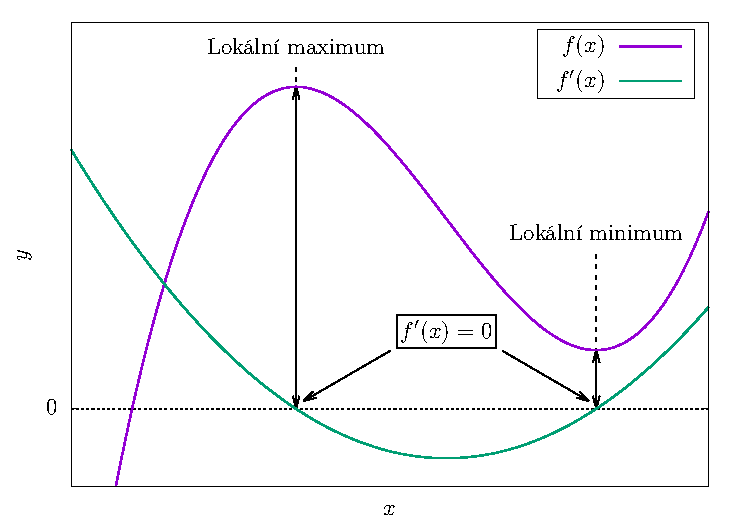
\includegraphics[scale = 0.7]{Gnuplot/Figures/funkce-derivace.pdf}
    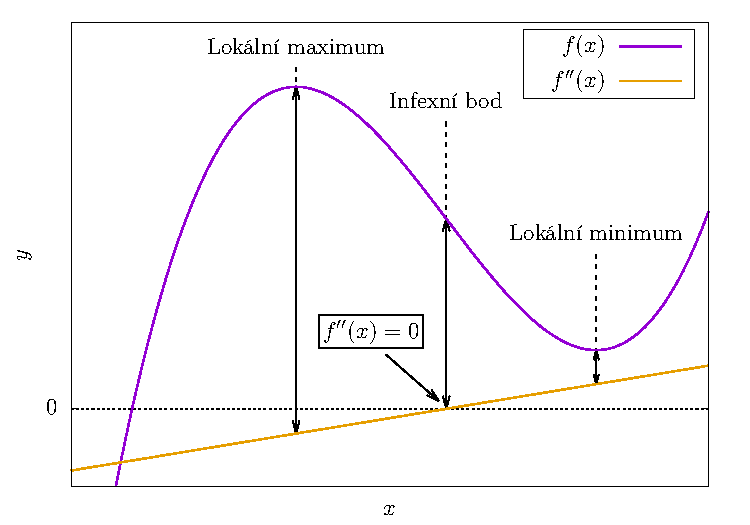
\includegraphics[scale = 0.7]{Gnuplot/Figures/funkce-druha-derivace.pdf}
    \caption{Ilustrace průběhu funkce, její první a druhé derivace.}
\end{figure}
\begin{table}[H]
    \centering

    \begin{tabular}{|c|c|c|}
        \hline
        vlastnost funkce & první derivace & druhá derivace \\
        \hline
        rostoucí & $+$ & jakákoli \\
        klesající & $-$ & jakákoli  \\
        konvexní & jakákoli & $+$ \\
        konkávní & jakákoli & $-$ \\ \hline
    \end{tabular}
    \caption{Charakterizace funkce podle první a druhé derivace.}
\end{table}

\begin{table}[H]
    \centering

    \begin{tabular}{|c|c|c|}
        \hline
        speciální bod & první derivace & druhá derivace \\
        \hline
        lokální minimum & $0$ & $+$ \\
        lokální maximum & $0$ & $-$ \\
        sedlový bod & $0$ & $0$ \\
        inflexní bod & jakákoli & $0$ \\ \hline
    \end{tabular}
    \caption{Charakterizace speciálních bodů funkcí. (U sedlového bodu nejsou podmínky postačující.)}
\end{table}

\section{Příklady}

\begin{example}
   

\end{example}

\section{Aplikované příklady}

\begin{example}[Maximální profit]
    Dejme tomu, že náklady $TC$ na výrobu produktu o množství $Q$ jsou dány funkcí 
    \begin{align}
        TC (Q) = 2 Q^3 - 3 Q^2 + 400 Q + 5000 
    \end{align}
    a cena produktu $P$ je dána funkcí \begin{align}
        P(Q) =  4000 - 33 Q \:.
    \end{align}
    Profitová funkce $\Pi$ (čti \uv{velké pí}) je dána rozdílem celkového příjmu a celkového nákladu
    \begin{align}
        \Pi = TR - TC \:, \quad \text{kde} \quad TR = P \cdot Q \:.
    \end{align} 
    Určeme maximální profit.

    Platí \begin{align}
        \Pi(Q) = 4\,000 Q - 33 Q^2 - 2 Q^3 + 3 Q^2 - 400 Q - 5\,000 = - 2 Q^3 - 30 Q^2 + 3\,600 Q - 5\,000\:.
    \end{align}
    Naším úkolem je nalézt maxima a minima takové funkce. K tomu spočteme derivaci
    \begin{align}
        \Pi'(Q) = - 6Q^2 - 60 Q + 3\,600
    \end{align}
    a určíme její nulové body $Q_0$. Musíme tedy vyřešit rovnici 
    \begin{align}
        Q_0^2 + 10 Q_0 - 600 = 0\:,
    \end{align}
    což není žádný problém:
    \begin{align}
        Q_0 = \frac{-10 \pm \sqrt{100 + 2\,400}}{2} = - 5 \pm 25 = -30 \:, \: +20 \:. 
    \end{align}
    Zjevně nás zajímá bod $Q_0 = 20$. Pomocí druhé derivace ověříme, o jaký stacionární bod se jedná.
    \begin{align}
        \Pi''(Q) = - 12 Q - 60 \:, \quad \Pi''(Q_0) = - 12 \cdot 20 - 60 < 0 \:,
    \end{align}
    takže se jedná o lokální maximum.

    Maximální profit tedy nastává při množství $Q_0 = 20$ a je roven 
    \begin{align}
        \Pi_{\text{max}} 
    = \Pi(Q_0) = -2 \cdot 20^3 - 30 \cdot 20^2 + 3600 \cdot 20 - 5\,000 = 39\,600 \:.
    \end{align}
\end{example}